\documentclass{beamer}
% Replace the \documentclass declaration above
% with the following two lines to typeset your 
% lecture notes as a handout:
%\documentclass[handout]{beamer}
\usepackage{CJKutf8}
\usepackage[T1]{fontenc}
%\usepackage[utf8x]{inputenc}
\usepackage{graphicx}
\usepackage{subfigure}
\usepackage{mathtools}
\usepackage{ulem}
\usepackage{url}
\usepackage{pifont}
\usepackage{pgfplots}
\usepackage{textcomp}

\usepgfplotslibrary{external}
\pgfplotsset{width=10cm,compat=1.9}

%% \usepackage{tikz}
%% \usepackage{verbatim}
%% \usepackage[active,tightpage]{preview}
%% \PreviewEnvironment{center}
%% \setlength\PreviewBorder{10pt}

\usetikzlibrary{shapes,arrows}

\tikzexternalize
\everymath{\displaystyle}

% There are many different themes available for Beamer. A comprehensive
% list with examples is given here:
% http://deic.uab.es/~iblanes/beamer_gallery/index_by_theme.html
% You can uncomment the themes below if you would like to use a different
% one:
%\usetheme{AnnArbor}
%\usetheme{Antibes}
%\usetheme{Bergen}
%\usetheme{Berkeley}
%\usetheme{Berlin}
%\usetheme{Boadilla}
%\usetheme{boxes}
%\usetheme{CambridgeUS}
%\usetheme{Copenhagen}
%\usetheme{Darmstadt}
%\usetheme{default}
%\usetheme{Frankfurt}
%\usetheme{Goettingen}
%\usetheme{Hannover}
%\usetheme{Ilmenau}
%\usetheme{JuanLesPins}
%\usetheme{Luebeck}
%\usetheme{Madrid}
%\usetheme{Malmoe}
%\usetheme{Marburg}
%\usetheme{Montpellier}
%\usetheme{PaloAlto}
%\usetheme{Pittsburgh}
%\usetheme{Rochester}
%\usetheme{Singapore}
%\usetheme{Szeged}
\usetheme{Warsaw}

%% \newcommand{chartnumproducts} {
%% }



\begin{document}

\begin{CJK}{UTF8}{gbsn}

\title{基于特征匹配的个性化推荐}

% A subtitle is optional and this may be deleted
\subtitle{个性化标签效果评估}

\author{李庚\inst{1}}
% - Give the names in the same order as the appear in the paper.
% - Use the \inst{?} command only if the authors have different
%   affiliation.

\institute[Qunar.com] % (optional, but mostly needed)
{
  \inst{1}
  旅游度假事业部-搜索及频道 \\
  Qunar.com
}
% - Use the \inst command only if there are several affiliations.
% - Keep it simple, no one is interested in your street address.

\date{\today}

\begin{frame}
  \titlepage
\end{frame}

\begin{frame}{基于特征匹配的推荐}

  $$ A \rightarrow x, B \rightarrow x $$
  $$ A \rightarrow y, C \rightarrow z $$
  $$ B \Leftarrow {\color{blue}{y}},z ? $$

  \begin{itemize}
  \item { A和B具有共同偏好特征$ u_1 $ }
  \item { 产品x具有特征 $ p_1 $ }
  \item { 具有 $ u_1 $ 特征的人偏爱具备 $ p_1 $ 特征的产品 }
  \item { 产品y也具有特征 $ p_1 $ }
  \end{itemize}

  \uncover <2-> { $ p_1 $特征即为推荐给B的理由,展示在list页 }

\end{frame}


\begin{frame}{排序加权并增加标签提示}
  \begin{columns}
    \begin{column}{0.4\textwidth}
      \begin{itemize}
      \item <2-> {
        特征选择:
        \begin {enumerate}
        \item { 住宿靠近景区 }
        \item { 住宿靠近地铁 }
        \item { 住宿靠近火车站}
        \item { 错峰出行 }
        \item { 住知名酒店 }
        \item { 住热门商圈 }
        \end {enumerate}
      }
      \end{itemize}
    \end{column}
    \begin{column}{0.6\textwidth}
      \begin{center}
        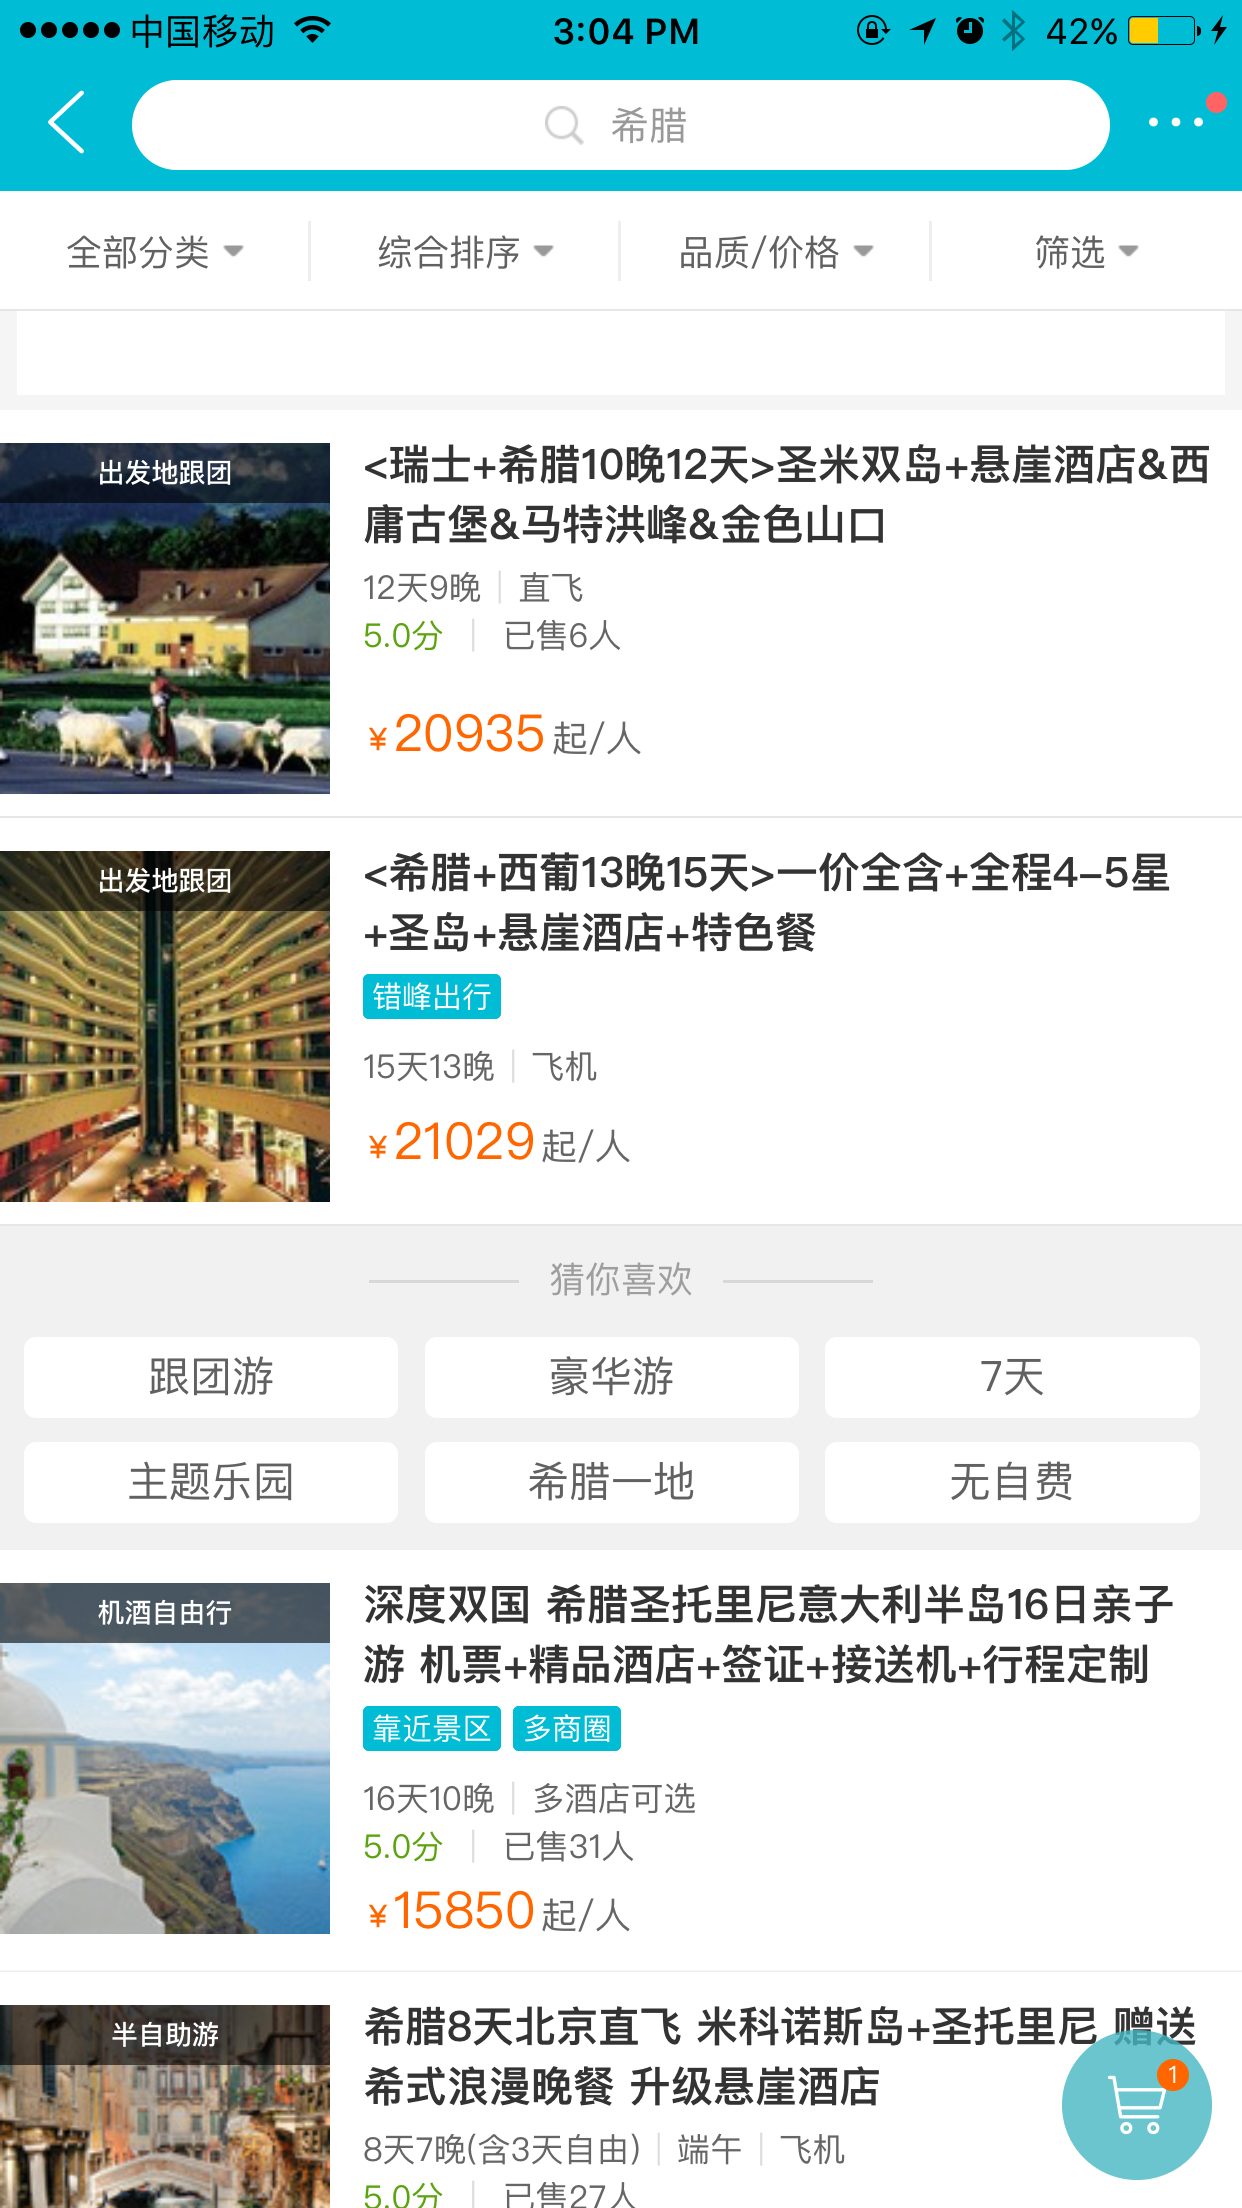
\includegraphics[scale=0.09]{./images/lables-demo.jpg}
      \end{center}
    \end{column}
  \end{columns}
\end{frame}

\begin{frame}{效果数据}
  \begin{enumerate}
  \item {覆盖用户比例:14.6\%}
  \item {
    iOS uv维度L-O转化率:
    \begin{itemize}
    \item { 置顶环境:0.0133 }
    \item { 个性化环境:0.0127 }
    \end{itemize}
    以上数据统计自3/9-3/17
  }
  \item {
    有标签vs无标签产品的转化率
    \begin{itemize}
    \item { L-D: 0.606 vs 0.510 }
    \item { D-O: 0.011 vs 0.007}
    \end {itemize}
  }
  \end{enumerate}
\end{frame}


\end{CJK}

\end{document}
